\documentclass[tikz,border=12pt]{standalone}
\usepackage[T1]{fontenc}
\usepackage{mathpazo}
\usepackage{amsmath,amssymb}
\usetikzlibrary{arrows.meta, positioning, calc, fit, decorations.pathreplacing}

\definecolor{stblue}{HTML}{7B97AD}
\definecolor{rwgold}{HTML}{B8995E}
\definecolor{sage}{HTML}{7A9A7E}
\definecolor{dkbrown}{HTML}{3D3530}
\definecolor{wmgray}{HTML}{7B7067}
\definecolor{cream}{HTML}{F9F6F0}
\definecolor{border}{HTML}{D4C9B8}
\definecolor{terracotta}{HTML}{C47A6A}
\definecolor{lavender}{HTML}{907EA0}

\begin{document}
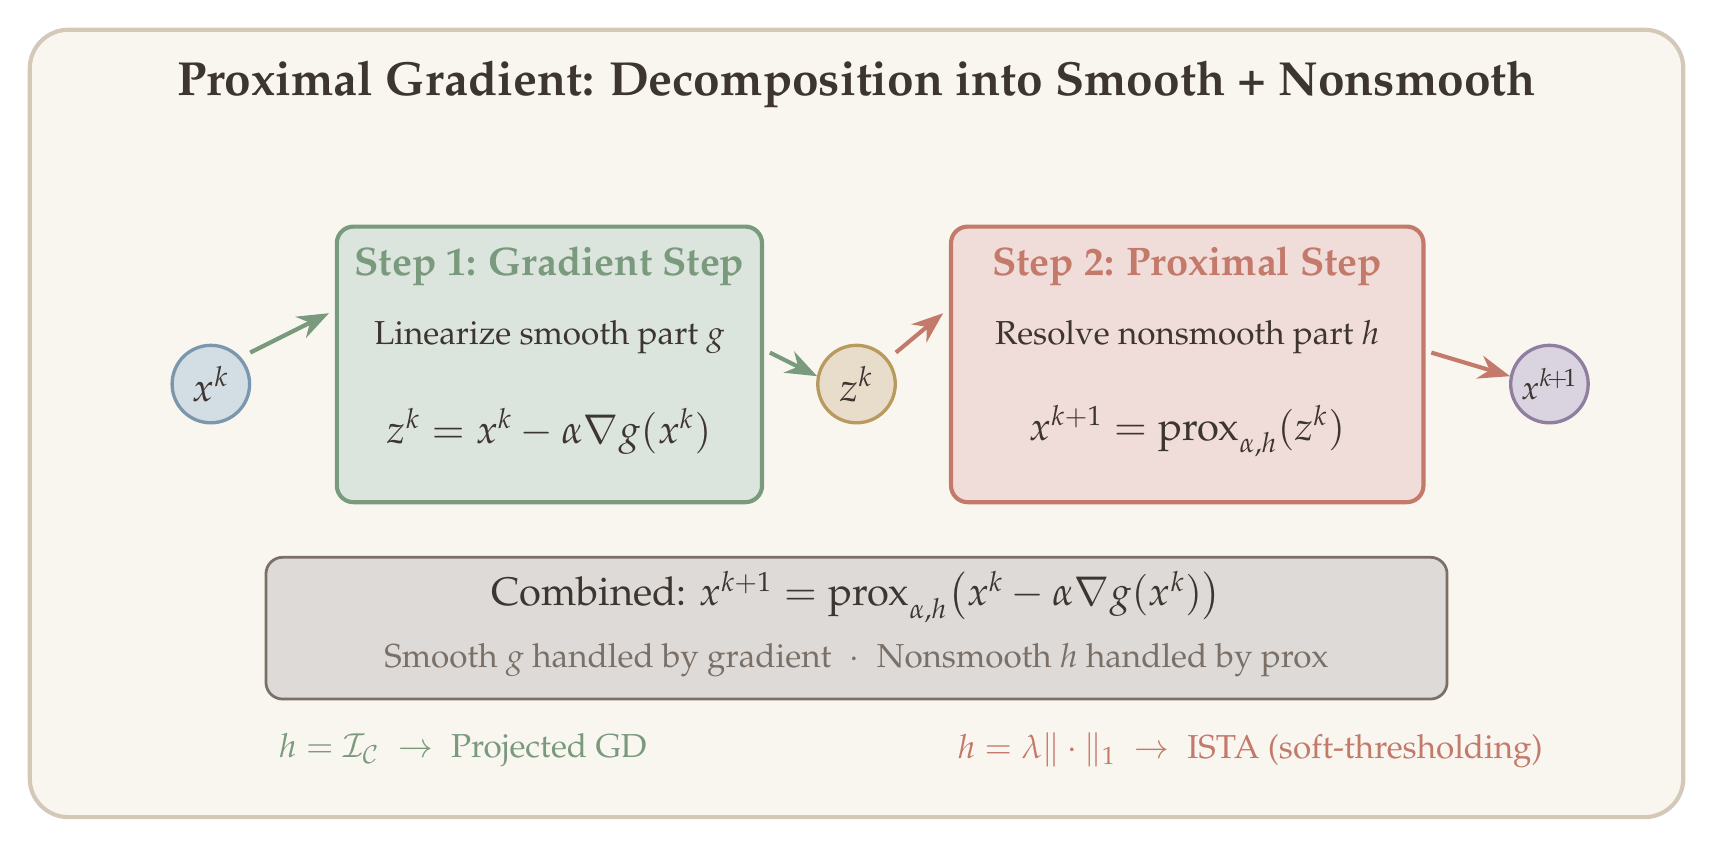
\begin{tikzpicture}[>={Stealth[length=4mm, width=3mm]}]

% Background
\fill[cream, rounded corners=14pt] (-0.5,-0.5) rectangle (20.5,9.5);
\draw[border, line width=1.5pt, rounded corners=14pt] (-0.5,-0.5) rectangle (20.5,9.5);

% Title
\node[text=dkbrown, font=\LARGE\bfseries] at (10,8.8) {Proximal Gradient: Decomposition into Smooth + Nonsmooth};

% Node: x^k
\fill[stblue!33] (1.8,5.0) circle (14pt);
\draw[stblue, line width=1.2pt] (1.8,5.0) circle (14pt);
\node[text=dkbrown, font=\Large] at (1.8,5.0) {$x^k$};

% Step 1: Gradient step box
\fill[sage!26, rounded corners=6pt] (3.4,3.5) rectangle (8.8,7.0);
\draw[sage, line width=1.5pt, rounded corners=6pt] (3.4,3.5) rectangle (8.8,7.0);
\node[text=sage, font=\Large\bfseries] at (6.1,6.5) {Step 1: Gradient Step};
\node[text=dkbrown, font=\large] at (6.1,5.6) {Linearize smooth part $g$};
\node[text=dkbrown, font=\Large] at (6.1,4.4) {$z^k = x^k - \alpha\nabla g(x^k)$};

% Arrow from x^k to step 1
\draw[sage, line width=1.5pt, ->] (2.3,5.4) -- (3.3,5.9);

% Node: z^k
\fill[rwgold!33] (10.0,5.0) circle (14pt);
\draw[rwgold, line width=1.2pt] (10.0,5.0) circle (14pt);
\node[text=dkbrown, font=\Large] at (10.0,5.0) {$z^k$};

% Arrow from step 1 to z^k
\draw[sage, line width=1.5pt, ->] (8.9,5.4) -- (9.5,5.1);

% Step 2: Prox step box
\fill[terracotta!26, rounded corners=6pt] (11.2,3.5) rectangle (17.2,7.0);
\draw[terracotta, line width=1.5pt, rounded corners=6pt] (11.2,3.5) rectangle (17.2,7.0);
\node[text=terracotta, font=\Large\bfseries] at (14.2,6.5) {Step 2: Proximal Step};
\node[text=dkbrown, font=\large] at (14.2,5.6) {Resolve nonsmooth part $h$};
\node[text=dkbrown, font=\Large] at (14.2,4.4) {$x^{k+1} = \operatorname{prox}_{\alpha,h}(z^k)$};

% Arrow from z^k to step 2
\draw[terracotta, line width=1.5pt, ->] (10.5,5.4) -- (11.1,5.9);

% Node: x^{k+1}
\fill[lavender!33] (18.8,5.0) circle (14pt);
\draw[lavender, line width=1.2pt] (18.8,5.0) circle (14pt);
\node[text=dkbrown, font=\large] at (18.8,5.0) {$x^{k\!+\!1}$};

% Arrow from step 2 to x^{k+1}
\draw[terracotta, line width=1.5pt, ->] (17.3,5.4) -- (18.3,5.1);

% Combined formula at bottom
\fill[wmgray!26, rounded corners=6pt] (2.5,1.0) rectangle (17.5,2.8);
\draw[wmgray, line width=1pt, rounded corners=6pt] (2.5,1.0) rectangle (17.5,2.8);
\node[text=dkbrown, font=\Large] at (10.0,2.3) {Combined: $x^{k+1} = \operatorname{prox}_{\alpha,h}\bigl(x^k - \alpha\nabla g(x^k)\bigr)$};
\node[text=wmgray, font=\large] at (10.0,1.5) {Smooth $g$ handled by gradient $\;\cdot\;$ Nonsmooth $h$ handled by prox};

% Bottom: special cases
\node[text=sage, font=\large] at (5.0,0.35) {$h = \mathcal{I}_{\mathcal{C}} \;\to\;$ Projected GD};
\node[text=terracotta, font=\large] at (15.0,0.35) {$h = \lambda\|\cdot\|_1 \;\to\;$ ISTA (soft-thresholding)};

\end{tikzpicture}
\end{document}
